%% how will i tackle the problem with justifications 
%% based on ideas in BACKGROUND

\chapter{Implementation}\label{ch:impl}

\section{Matlab implementation of neural network} \label{se:impl.matlab.nn}

There are several motivations for choosing this particular implementation of neural network as a reference point. First, Matlab implementation is heavily reliant upon the mathematical interpretation of neural network and is clearly understandable where matrix multiplication and vectorisation is concerned. It was projected that it would be fairly simple and in the closest in spirit implementation to how it may work in Accelerate due to this.

Secondly, the Matlab implementation had a certain data set with expected 'answers' to compare my own implementations to. Thus, I could be assured that my implementation in Accelerate was accurate enough to be reliable, particularly in the light of difficulty of debugging Accelerate programs. Passing this 'accuracy' test will prove the small network reliable enough to be built upon for further development in the future.

Thirdly, the codebase that I am basing my program is from Coursera, an online self-learning course, made by Andrew Ng of Stanford University. This course has drawn wide praise for its material and presumed to be reviewed by many in the same field. The structure of the course is reliable in terms of correctness and efficiency, and implemented already with much knowledge in the field. Hence, I projected that the Matlab implementation would be optimised for the best performance.

Lastly, in terms of familiarity, I was more conversed with Matlab than with other neural network implementations, such as Python, C++, or Haskell, (PUT REFERENCES TO THESE IMPLEMENTATIONS) which may needlessly increase the time to start the project. I had researched about other implementations, but found that it took more time to understand these in order to integrate or implement an Accelerate neural network.

TO CHECK::::: Can C++ or Python versions use multiple threads/GPU?

\subsection{Peculiarities of Matlab} \label{se:impl.matlab.background}
%% or divide this up into implementation section

MATLAB, or Matrix Laboratory, is a highly doman-specific programming language, specialised to conduct numerical calculations and analysis in late 1970s. It is a imperative, object-orientated, procedural language. It is widely used among the industry and academia, particularly in science, engineering and economics.

MATLAB is a weakly typed programming language, as types are implicitly converted~\cite{Wiki1}. This means that variables can be declared without an explicit declaration of their type. Furthermore, MATLAB is also dynamically typed, meaning that the types may also change during runtime. All variables in MATLAB are "structure arrays", that is, each element of the array have the same fields. 

MATLAB functions accept matrices as an argument, and will automatically apply multiplications of a scalar to each element of the matrix as in Accelerate's \texttt{zipWith}. As a result, MATLAB code is deceptively simple and does not reveal the actual structure of the underlying operation. Indexing of matrices and arrays also start from 1. Method dispatching also does not strictly adhere to the method signature, but selects the method by first matching the arguments in a class precedence and then by left-most priority~\cite{Mat17}. However, MATLAB also does not support overloading functions of the same name using different signature of the same name.

\section{Accelerate Implementation} \label{se:impl.acc}

\subsection{Neural network structure} \label{se:impl.nn.struct}

A 3-layer simple neural network is implemented, with an input layer, hidden layer and an output layer. There is an bias unit which always outputs $+1$ in each preceding layer to the next. 

My implementation can easily be modified to take more than 1 hidden layer by changing the \texttt{nnCostFunction}~\ref{fig:nnCostFunction.hiddenlayers}. For instance, each extra hidden layer should only require implementing two extra matrix multiplications in feed-forward and backpropagate, and all the steps required to update the new theta layer calculations.

\begin{figure}
  \begin{lstlisting}
    -- current feed-forward with 1 hidden layer
    a3 :: Acc (Matrix Float)
    a1 = xs 
    z2 = theta1 <> transpose a1 
    a2 = (fill (lift (Z :. h :. constant  1)) 1 :: Acc (Matrix Float)) 
         A.++ (A.transpose $ A.map sigmoid z2) 
    z3 = a2 <> A.transpose theta2 
    a3 = A.map sigmoid z3
    
    -- an example feed-forward with 2 hidden layers
    a4 :: Acc (Matrix Float)
    a3' = (fill (lift (Z :. h' :. constant  1)) 1 :: Acc (Matrix Float))
          A.++ (A.transpose $ A.map sigmoid z3)
    z4 = a3' <> A.transpose theta3
    a4 = A.map sigmoid z4
    
    -- an example backpropagate with 2 hidden layers
    d4 = A.zipWith (-) a4 ys
    d3 = A.zipWith (*) 
         (d4 <> theta3)
         ((fill (lift (Z :. h' :. constant  1)) 1 :: Acc (Matrix Float)) 
           A.++ (A.transpose $ A.map sigmoidGradient z3)) 
    d2 = A.zipWith (*) 
         (d3 <> theta2)
         ((fill (lift (Z :. h :. constant  1)) 1 :: Acc (Matrix Float)) 
           A.++ (A.transpose $ A.map sigmoidGradient z2)) 
  \end{lstlisting}
  \caption{Changing the number of hidden layers in \texttt{nnCostFunction}}
  \label{fig:nnCostFunction.hiddenlayers}
\end{figure}

The hidden layer in the handwritten numbers example roughly corresponds to detectors that look for strokes and other patterns in the input~\cite{Ng12}.

\subsection{Program structure} \label{se:impl.program.struct}

I have constructed my program to closely follow the MATLAB implementation. It can be preportioned into 3 parts: (1) initialisation; (2) neural network cost function; and, (3) function minimise conjugate gradient function. These will be explained in detail in the sections below.

\subsection{Initialisation} \label{se:impl.init}

Initialisation is a straightforward process, and we initialise (1) the learning rate \texttt{lambda}; (2) initial weight vectors, for instance \texttt{theta1}, \texttt{theta2}; (3) size of the input, hidden, output layers; and, (4) load the training set, that is, the input data set \texttt{xs} and the output data vector \texttt{ys}. 

\texttt{xs} represents $m$ training set data. After it has been loaded, each row of \texttt{xs} should represent a single training example, $x_1, x_2, ..., x_m$ where the length of $x_i$ is the size of the input layer. , with a column vector of $1$s to the leftmost of the array to represent the bias neuron,
\[
 \texttt{xs} =
    \begin{bmatrix}
      1 \\
      1 \\
      ... \\ 
      1
    \end{bmatrix}
    \begin{bmatrix}
       x_1 \\
       x_2 \\
       ... \\
       x_m
    \end{bmatrix}
\]

For the weights, the values should be in the range $[-\epsilon_{init}, \epsilon_{init}]$ for an effective random initialisation~\cite{Ng12}. One effective choice of $\epsilon_{init}$ is,
\[ \epsilon_{init} = \sqrt{\frac{6}{L_{in} + L_{out}}} \]
where $L_{in}$ is number of units in the preceding layer, and $L_{out}$ is the number of units in the subsequent layer of the thetas in question. 

There is no optimal $\lambda$, or learning rate value. Generally, the one that gives the best result for the given data set is determined by trial-and-error. Likewise, the number of hidden units and even the number of hidden layers also seems to be determined by trial-and-error.

The numbers for the input and output units correspond to the number of attributes in the samples and the number of classifications that these samples should be divided into.

\subsection{Neural network cost function} \label{se:impl.nnCostFunction}

This function implements both the feed-forward and back-progapation to a sample data input in the existing neural network system and updates the weight vectors and error costs accordingly. It includes application of sigmoid function and regularisation calculation. 

However, instead of parsing each sample data one-by-one, following the style of MATLAB implementation, it groups all of the sample data into one massive matrix to parse them in all at once in bulk. 

CHECK IF THIS IS CORRECT::: Although this batch sample method is less accurate than if the examples were parsed in one by one, it is much more time efficient.

The Accelerate implementation of this was also straightforward as this function only requires reshaping of the vectors, implemented using \texttt{reshape}, matrix multiplications, at first using \texttt{mmult}, eventually replaced with \texttt{INSERT NAME OF NEW MATRIX MULTIPLIER HERE} which has better performance. Other arithmetic operations were applied to matrixes coupled with \texttt{map} and \texttt{zipWith}.

As Accelerate has its own sets of arithmetic operations, any calculations that were needed in the Accelerate world was using the Accelerate version, marked with \texttt{A}. The Haskell world version was marked with \texttt{P} for \texttt{Prelude}.

PUT EXAMPLE HERE 

For the full functions, please refer to Appendix 1~\ref{fig:nnCostFunction.matlab}, ~\ref{fig:nnCostFunction.acc}

\begin{figure}
	\centerline{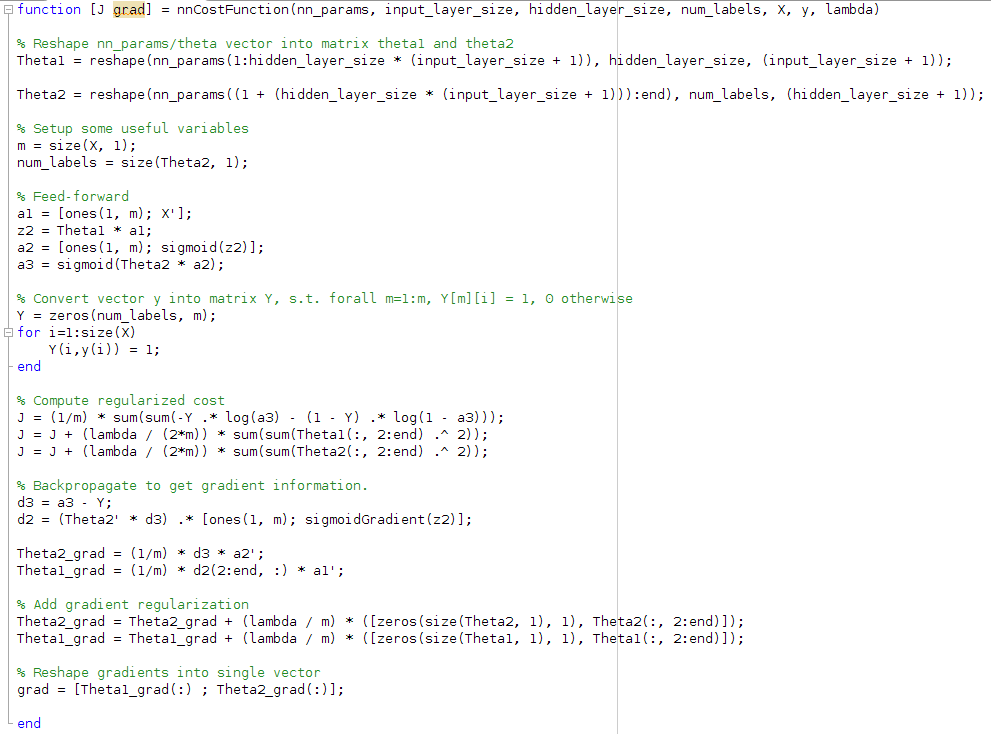
\includegraphics[width=\linewidth]{nnCostFunction-matlab.png}}
	\caption{Neural network cost function in Matlab.}
	\label{fig:nnCostFunction.matlab}
\end{figure}

\begin{figure}
	\centerline{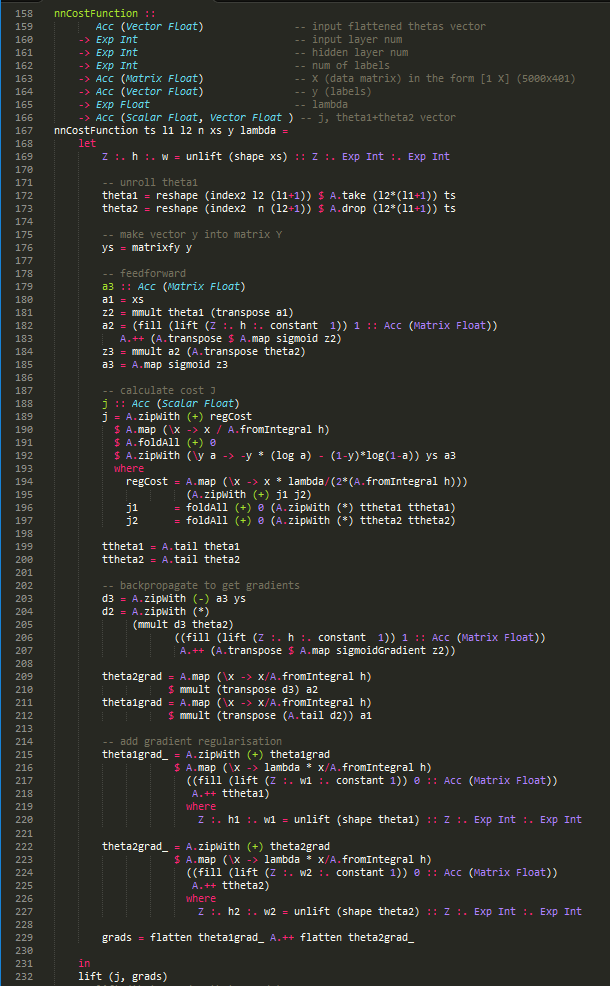
\includegraphics[width=\linewidth]{nnCostFunction-acc.png}}
	\caption{Neural network cost function in Accelerate.}
	\label{fig:nnCostFunction.acc}
\end{figure}

\subsection{Function minimise nonlinear conjugate gradient function} \label{se:impl.fmincg}

This function is a modified version of MATLAB's \texttt{fminunc}. Given 
$$\texttt{x = fminunc(func, x0)}$$
\texttt{x} is the the local minimum of unconstrained multivariate function \texttt{func}, from starting point \texttt{x0}. \texttt{x0} can be a scalar, vector or a matrix.~\cite{Reb13}

\texttt{fmincg} is a more efficient modification of \texttt{fminunc} to minimize a continuous differentialble multivariate function. It uses Polack-Ribiere flavour of conjugate gradients, quadratic and cubic polynomial approximations and the Wolfe-Powell stopping criteria to more efficiently calculate slope and stepping sizes~\cite{Mat17}. The mathematics behind applying these methods are beyond the scope of this project.

The function terminates when it either finds the local minimum, or if the progress is so non-significant that it is not worth any further exploration. It returns the solution vector as \texttt{X} and the cost vector \texttt{fX}, which indicates the cost of each iteration or the progress made.

Translating \texttt{fmincg} into Accelerate is tricky. First, the MATLAB code had around 17 parameters, all of which constantly updated their values in a procedural way. Without a knowledge of the underlying mathematics, the procedure was puzzling. Their non-descript names, such as, \texttt{d1, f1, v1} were not enlightening either. Overall, it was difficult to follow the flow of control. I thus have followed the flow of procedure very closely, albeit with some substitions, as there were some aspects that were not yet implemented in Accelerate, such as \texttt{isInfinite} and \texttt{isNaN}. 

Second, there were three \texttt{while} loops in this code, with three \texttt{if-else} statements, one which had a flow divergence. Due to this, the type of flat parallelism may not be best suited for the GPU, although the flow divergence was upon a failure to find local minimum - which happens when the function supplied to \texttt{fmincg} is inaccurate~\cite{Reb13}. Thus, to get rid of this flow divergence, I have taken the assumption that there is always a local minimum that \texttt{fmincg} can  find, because the function supplied can be checked to be accurate prior to being supplied to this function.

Also, due to the limitations of MATLAB in \texttt{fmincg}, there is a seemingly redundant step of flattening the initial weight matrices into a vector, passing it as a parameter into \texttt{fmincg}. It is promptly then unrolled back into their original matrix shape, and after all the operations inside this function is complete, it is reflattened into a vector and returned.

This is to enable the function to iterate regardless of the matrices' size or shape. This duty is pushed to the function.

The MATLAB version of the code had approximately 175 lines. I divided these up into their \texttt{while} loops and connected the parts using Accelerate's \texttt{awhile} flow control. This required \texttt{lift}, \texttt{unlift} in order to pack and unpack the many variables into a single \texttt{Acc} tuple in order to be passed around the loop. Through this process, I learnt that Accelerate cannot infer the type unless if the \texttt{unlift}ed expression is used, and it is thus sometimes necessary to predefine types for certain terms.

Accompanying this issue was that \texttt{awhile} requires that set of results I need after the \texttt{while} loop finishes be part of the tuples wrapped in \texttt{Acc}. This meant that even the paramters that are not used needed to be packed together, and these always needed a help in type inference as Accelerate could not infer their types during the loop.

GIVE EXAMPLES

Such an implementation could be considered inefficient due to the number of space it consumes memory by creating intermediate variables rather unnecessarily in other languages. This has less impact with Accelerate due to 'sharing recovery', which will be explained in \ref{se:impl.benefits}.

\section{Limitations of this implementation} \label{se:impl.limits}

There are several issues with my Accelerate implementation. For one, there are a couple of functions which may not cover all the cases that MATLAB implementation may cover. For example, \texttt{fmincg} requires to optimise and to take care of cases where certain variables are \texttt{isinf}, \texttt{isreal} or \texttt{isnan}, that is, whether a variable has an infinite value, is a real number, or is not-a-number correspondingly. Since these are yet to be implemented in Accelerate, I have substituted them for when an determinate may be less than zero for \texttt{isreal}, divisor is 0 for \texttt{isnan} and ignored the case for \texttt{isinf}. This may not cover all the range of numbers.

Secondly, Matlab's \texttt{double} is by default a double-precision data type, and requires 64 bits~\cite{Mat17}. Yet, after testing it on the sample data, using \texttt{double} produces a result further away from the expected result than had I parsed them in Accelerate as \texttt{float}. This is a problem, because it may lead to inaccuracy. Also, one part in the MATLAB code accounts for overflow it seems, by minusing a \texttt{realmin} from a dividend,

$$-- PUT EXAMPLE HERE$$

but \texttt{realmin} for \texttt{Float} is $1.1755e^{38}$ and for a \texttt{Double} is $2.2251e^{308}$, which are orders of magnitude of $1xe^{270}$ times different and could vastly affect the result.

Lastly, some of the optimisations in \texttt{fmincg} to come to the conclusion faster has been ignored, namely, the innermost loop and the handling a failure to obtain an answer. The reasons for this is that failure should not be triggered if the function input is valid and it needlessly slows down the software by introducing flow divergence. Also, the innermost loop does not behave in the expected manner and the reasons for this is still unfathomed at the time of writing the thesis.

Also because this implementation is more or less a straight forward translation of MATLAB code with minimal optimisation to suit Accelerate, there may be even more faster and efficient manner to create a neural network in native Accelerate, particularly in regards to \texttt{fmincg}.

